%!TEX root = ../thesis.tex
%*******************************************************************************
%****************************** Third Chapter **********************************
%*******************************************************************************
\chapter{Protocols and analysis of single-cell DNA methylation data} \label{sec:pro}

% **************************** Define Graphics Path **************************
\ifpdf
    \graphicspath{{Chapter3/Figs/Raster/}{Chapter3/Figs/PDF/}{Chapter3/Figs/}}
\else
    \graphicspath{{Chapter3/Figs/Vector/}{Chapter3/Figs/}}
\fi

Our undestanding of DNA methylation has been revolutionized by the development of BS-seq, which offers single-cytosine resolution and absolute quantification of 5mC genome-wide. Recent advances have demonstrated the power of single-cell sequencing to deconvolve mixed cell populations~\citep{jain_supervised_2007,deng_single-cell_2014,macaulay_single_2014}. Incorporating epigenetic information into this single-cell arsenal will provide insights into epigenetic heterogeneity and transform our understanding of gene regulation.

In the first section of this chapter, we will describe the scBS-seq protocol for genome-wide profiling of DNA methylation in single cells, a statistical method for quantifying methylation variability between cells, and applications to mouse ESCs. The work is based on \citet{smallwood_single-cell_2014}, which was joint work of Sebastien Smallwood, Heather Lee, Christof Angermueller, Felix Krueger, Heba Saadeh, Julian Peat, Simon Andrews, Oliver Stegle, and Wolf Reik.

\begin{center}
\begin{minipage}{.9\linewidth}
\underline{Individual contributions}: Sebastien Smallwood and Heather Lee designed the study, prepared scBS-seq libraries, analysed data and wrote the manuscript. Felix Krueger, Heba Saadeh, and Sebastien Smallwood performed sequence mapping and analysed data. Julian Peat contributed to technical developments. Christof Angermueller and Oliver Stegle analysed the data.
\end{minipage}
\end{center}

In the second section, we will describe the scM\&T-seq protocol for parallel profiling of DNA methylation and gene expression in single cells, methods for quantifying associations between DNA methylation and gene expression, and applications to mouse ESCs. The work is based on \citet{angermueller_parallel_2016}, which was joint work of Christof Angermueller, Stephen Clark, Heather Lee, Iain Macaulay, Mabel Teng, Tim Xiaoming Hu, Felix Krueger, Sebastien Smallwood, Chris Ponting, Thierry Voet, Gavin Kelsey, Oliver Stegle, and Wolf Reik.

\begin{center}
\begin{minipage}{.9\linewidth}
\underline{Individual contributions}: Christof Angermueller performed all statistical analyses of the data. Heather Lee, Iain Macaulay, Stephen Clark, and Sebastien Smallwood developed the protocol and performed experiments. Heather Lee, Iain Macaulay, Christof Angermueller, Stephen Clark, Oliver Stegle, Wolf Reik, and Chris Ponting interpreted the results. Mabel Teng contributed to method development. Tim Xiaoming Hu processed RNA-seq data. Felix Krueger processed BS-seq data. Wolf Reik, Gavin Kelsey, Iain Macaula, and Thierry Voet contributed protocols and reagents. Heather Lee, Iain Macaulay, Wolf Reik, and Thierry Voet conceived the project.
\end{minipage}
\end{center}

\section{Estimating DNA methylation variability in embryonic stem cells} \label{sec:bs}

\ifpdf
    \graphicspath{{Chapter3/bs/Figs/Raster/}{Chapter3/bs/Figs/PDF/}{Chapter3/bs/Figs/}}
\else
    \graphicspath{{Chapter3/bs/Figs/Vector/}{Chapter3/bs/Figs/}}
\fi

Several protocols have been developed for profiling average DNA methylation levels of in bulk populations of cells (\Cref{sec:intro_proto}). However, bulk profiling protocols are unable to directly estimate methylation heterogeneity between single cells, which is critical for studying embryonic development, cancer progression, and pluripotent stem cells. In the following, we will describe scBS-seq, an accurate and reproducible method for profiling DNA methylation in single cells, and a statistical model for estimating methylation heterogeneity in cell populations across the entire genome.


\subsection{Single-cell bisulfite sequencing protocol} \label{sec:bs_proto}

In commonly used BS-seq protocols, sequencing adaptors are ligated to fragmented DNA before bisulfite conversion, which results in a loss of information owing to DNA degradation by the bisulfite treatment. To minimize DNA loss from single cells, we developed a modification of post-bisulfite adaptor tagging~\citep{miura_amplification-free_2012-1}. In scBS-seq, bisulfite treatment is performed first, which results in simultaneous DNA fragmentation and conversion of unmethylated cytosines to thymine (\Cref{fig:bs_proto}). Then, synthesis of complementary strands is primed using oligonuleotides containing Illumina adaptor sequences and a 3' stretch of nine random nucleotides. This step is performed five times to maximize the number of tagged DNA strands and to generate multiple copies of each fragment. After capturing the tagged strands, a second adaptor is similarly integrated, and PCR amplification is performed with indexed primers.

\begin{figure}[htbp!]
\centering
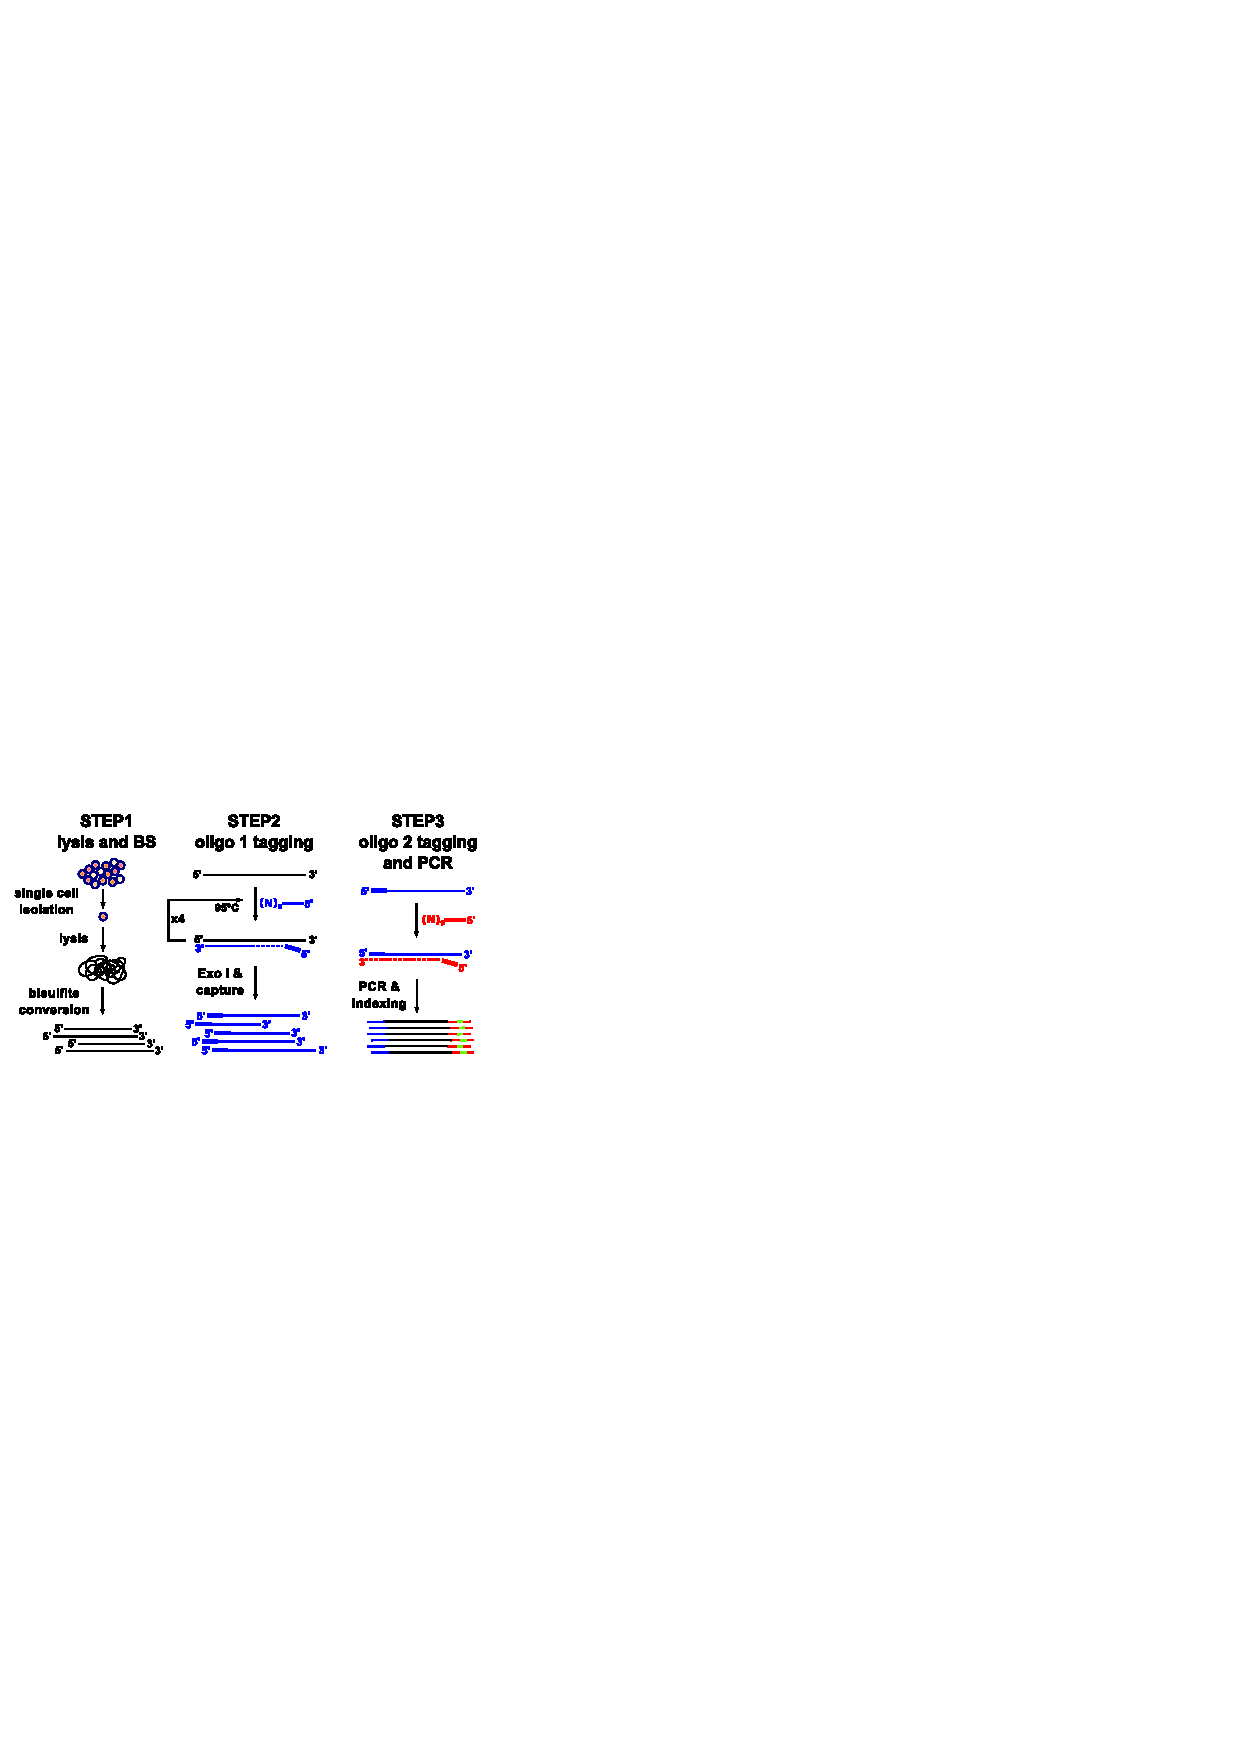
\includegraphics[width=0.75\textwidth]{proto}
\caption[scBS-seq profiling protocol.]{scBS-seq profiling protocol. scBS-seq library preparation consists of isolating and lysing single cells before bisulfite conversion (`BS'); performing five rounds of random priming and extension using oligo 1 (which carries the first sequencing adaptor) and purifying synthesized fragments; and performing a second random priming and extension step using oligo 2 (which carries the second sequencing adaptor) before amplifying the resulting fragments.}
\label{fig:bs_proto}
\end{figure}

We assessed scBS-seq on ovulated metaphase II oocytes (MIIs) and mouse ESCs cultured either in 2i medium or serum conditions. MIIs are a suited model for technical assessment as they: (i) can be individually hand- picked to ensure that only one cell is processed; (ii) represent a highly homogeneous population, which allows discrimination between technical and biological variability; and (iii) present a distinct DNA methylome comprising large-scale hypermethylated and hypomethylated domains~\citep{shirane_mouse_2013}. ESCs grown in serum conditions are characterized by a high heterogeneity in DNA methylation and gene expression and hence suited for the estimating of intercellular heterogenetiy~\citep{ficz_fgf_2013}. We used ESCs grown in serum (`serum ESCs') and ESCs grown in 2i medium (`2i ESCs') to determine whether scBS-seq can reveal DNA methylation heterogeneity in single cells.

We sequenced 12 MII, 12 2i ESC, 20 serum ESC, and 7 negative controls using scBS-seq, and their bulk cell counterparts using BS-seq. We obtained the methylation state of on average 3.7 million CpG dinucleotides (CpGs; range, 1.8 M–7.7 M) corresponding to 17.7\% of all CpGs (range, 8.5–36.2\%; \Cref{fig:bs_qc}~(a)). A higher CpG coverage can be obtained by deeper sequencing. To validate this, we sequenced two MII libraries close to saturation, which resulted in 1.5-fold and 1.9-fold more CpGs captured. Altogether, we obtained up to 10.1 M CpGs, corresponding to a CpG coverage of 48.4\%.

\begin{figure}[htbp!]
\centering
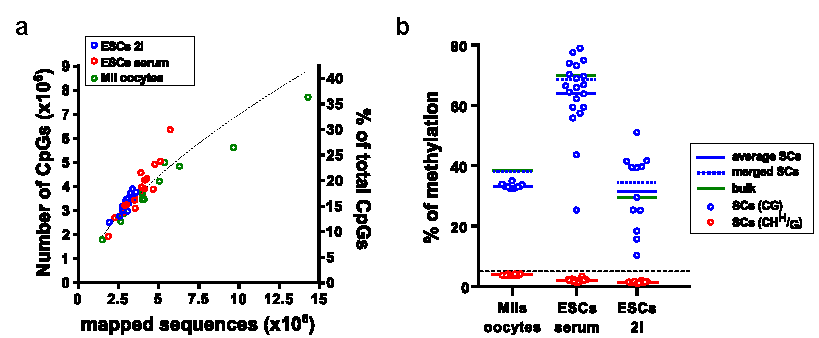
\includegraphics[width=0.8\textwidth]{qc}
\caption[scBS-seq mapping efficiency and mean methylation levels.]{scBS-seq mapping efficiency and mean methylation levels. (a) Number of CpGs obtained by scBS-seq as a function of mapped sequences. (b) Global mean DNA methylation levels in CpG (CG) and non-CpG (CHH/G) context for single cells (SCs), in silico–merged, and bulk samples. }
\label{fig:bs_qc}
\end{figure}

Next, we investigated the reproducibility and accuracy of scBS-seq. CpG sites in MIIs were overwhelmingly called methylated or unmethylated, which is consistent with a highly digitized output from single cells (\Cref{fig:bs_binary}). As expected, global methylation of MIIs was highly homogeneous ($33.1 \pm 0.8\%$) and 2i ESCs were hypomethylated compared to serum ESCs13. Yet both 2i ESCs and serum ESCs exhibited 5mC heterogeneity (serum, $63.9 \pm 12.4\%$; 2i medium, $31.3 \pm 12.6\%$; \Cref{fig:bs_qc}~(b)). We determined the average pairwise concordance between individual CpGs across single oocyte libraries, which was 87.6\% genome- wide (range, 85.3–88.9\%) and 95.7\% in unmethylated CGIs, a highly homogeneous genomic feature (\Cref{fig:bs_concord}~(a)). CpG concordance in ESCs was lower (serum, 72.7\%; 2i medium, 69.8\%), which reflected the heterogeneity of these cells (\Cref{fig:bs_concord}~(a)). At two kilo base pair (kbp) resolution, we observed high correlation between individual MIIs (Pearson's $r=0.92$), and between individual MIIs and bulk (Pearson's $r=0.95$) (\Cref{fig:bs_concord}~(b)). We could largely reproduce the entire bulk methylation profile of oocytes using only 12 single cells (\Cref{fig:bs_concord}~(b)). This capability is particularly beneficial for analyses of homogeneous cell populations and makes scBS-seq an important tool to investigate the 5mC landscape in very rare material.

\begin{figure}[htbp!]
\centering
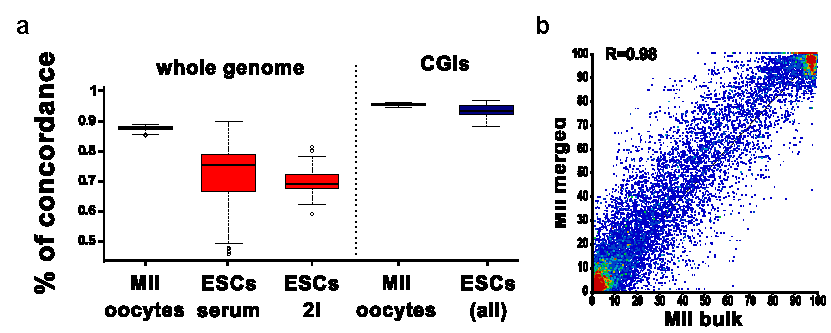
\includegraphics[width=1.0\textwidth]{concord}
\caption[CpG concordance and reproduction of bulk data.]{CpG concordance and reproduction of bulk data. (a) Pairwise analysis of CpG concordance genome-wide and in unmethylated CGIs. Boxplots represent the interquartile range, with the median; whiskers correspond to 1.5 times the interquartile range. (b) Pairwise correlation CpG methylation levels between MII-merged and MII-bulk data.}
\label{fig:bs_concord}
\end{figure}


\subsection{Method for estimating DNA methylation variability} \label{sec:bs_method}

The majority of CpG sites in single cells are either methylated or unmethylated. An exception is hemimethylation, where the cytosine is methylated on only one DNA strand. Consistent with this, scBS-seq called CpG sites overwhelmingly methylated or unmethylated (\Cref{fig:bs_binary}). Since hemimethylation is rare and currently hard to detect by scBS-seq owing to low CpG coverage, we did not consider hemimethylation in our analysis. Instead, we modelled the methylation state of CpG sites in single-cells as a Bernoulli variable, and represented methylation profiles as a binary matrix (\Cref{fig:bs_binary}). As a consequence of the limited CpG coverage of only ${\approx}10-30\%$, the methylation state of most CpG sites is unobserved, which renders downstream analyses challenging. We therefore developed a method that aggregates information from adjacent CpG sites and estimates mean methylation levels as well as cell-to-cell heterogeneity for windows instead of single CpG sites. Our method yields uncertainty estimates, which is critical in regions of low CpG coverage. Our method is further computational efficient, thereby applicable genome-wide on over 20 million CpG sites.

\begin{figure}[htbp!]
\centering
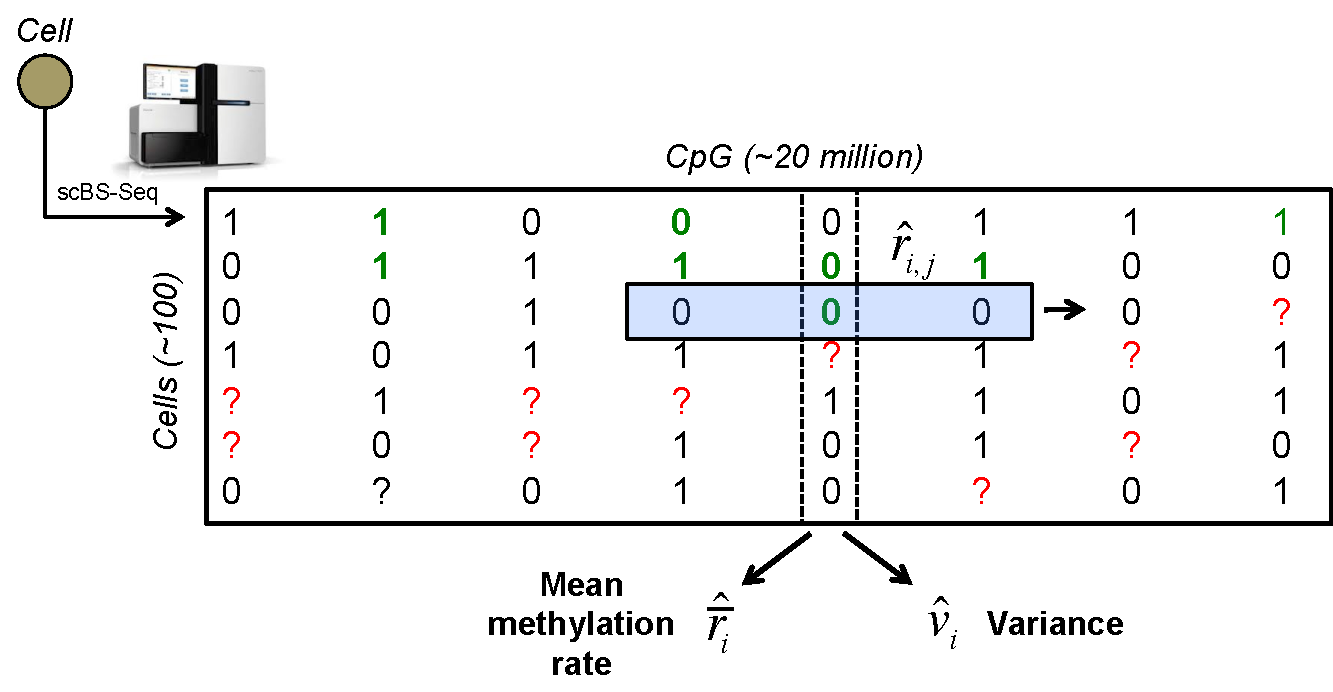
\includegraphics[width=0.9\textwidth]{method}
\caption[Representation of single-cell methylation data.]{Representation of single-cell methylation data. Binary matrix $M$ with rows corresponding to cells and columns to CpG sites. $M_{i,j}$ represent the methylation state of CpG site $i$ in cell $j$, which is one if the CpG site is methylated and zero otherwise. Question marks denote sites with unobserved methylation state. A sliding window (blue) is used to first estimate the methylation rate $\hat{r}_{i,j}$ (green) for each cell and window, and the mean methylation rate $\hat{\bar{r}}_i$ and variance $\hat{v}_i$ across cells afterwards.}
\label{fig:bs_method}
\end{figure}


\newcommand{\Xfw}{c^+}
\newcommand{\Xrv}{c^-}
\newcommand{\Xfws}{s^+_{i,j}}
\newcommand{\Xrvs}{s^-_{i,j}}
\newcommand{\XBin}{\operatorname{Bin}}
\newcommand{\Xse}{\operatorname{SE}}
\newcommand{\Xrij}{\hat{r}_{i,j}}
\newcommand{\Xri}{\hat{r}_i}
\newcommand{\Xwij}{w_{i,j}}
\newcommand{\Xrmi}{\hat{\overline{r}}_i}
\newcommand{\Xrvi}{\hat{v}_i}
\newcommand{\Xrvli}{\hat{v}^l_i}
\newcommand{\Xrvui}{\hat{v}^u_i}
\newcommand{\Xwjji}{w^{j,j^\prime}_i}


\subsubsection{Estimating cell-specific methylation rates}

To increase the coverage across cells, we employed a sliding window approach, which is conceptually similar to approaches that have been used for bulk BS-Seq~\citep{bock_dna_2012,li_dna_2010}. With window size $w=3000$~bp and step size 600~bp, we computed for each cell $j$ the sum of methylated $c^+_{i,j}$ and unmethylated $c^-_{i,j}$ read counts in window $i$:
\begin{align}
  \Xfws = \sum_{k=-w/2}^{+w/2} \Xfw_{i+k, j} \qquad
  \Xrvs = \sum_{k=-w/2}^{+w/2} \Xrv_{i+k, j}
\end{align}
To estimate methylation rates, we modelled the sum $S^+_{i,j}$ of methylated read counts as a Binomial random variable with methylation rate $r_{i,j}$:
\begin{align}
  S^+_{i,j}\sim \XBin(\Xfws+\Xrvs, r_{i,j})
\end{align}
Assuming $r_{i,j}\sim \operatorname{Beta}(1,1)$, leads to the maximum a posteriori estimator $\hat{r}_{i,j}$ of the methylation rate in cell $j$ and window $i$:
\begin{align}
  \Xrij = \frac{\Xfws+1}{\Xfws+\Xrvs+2}
\end{align}
To account for the limited CpG coverage of scBS-seq (\Cref{sec:bs_proto}), we quantified prediction uncertainty by approximating the standard error of the rate estimator using the Wald method~\citep{stein_sequential_1947}:
\begin{align}
  \Xse[\Xrij]^2 = \frac{\Xrij(1-\Xrij)}{\Xfws+\Xrvs}
\end{align}


\subsubsection{Estimating cell-to-cell variability}

We used the estimated cell-specific methylation rates $\Xrij$ to estimate the mean methylation rate and variance across all cells. We modelled the mean methylation rate $r_i$ in window~$i$ as a Gaussian random variable with mean $\overline{r}_i$ and variance $v_i$:
\begin{align}
  r_i \sim N(\overline{r}_i, v_i)
\end{align}
To account for differences in the standard errors $\Xse[\Xrij]$, we weighted cell $j$ and position $i$ by $\Xwij=\Xse[\Xrij]^{-2}$, and used the weighted maximum likelihood estimator
\begin{align}
  \Xrmi = \frac{1}{\sum_j \Xwij} \sum_j \Xwij\Xrij
\end{align}
to estimate $\overline{r}_i$. Its standard error is given by
\begin{align}
  \Xse[\Xrmi]^2 = \frac{1}{\sum_j \Xwij}.
\end{align}
The maximum likelihood estimator of the variance $v_i$ is
\begin{align} \label{eq:bs_var}
  \Xrvi = \frac{\sum_j \Xwij}{\left(\sum_j \Xwij\right)^2 - \sum_j \Xwij^2} \sum_j \Xwij \left(\Xrij - \Xrmi\right)^2,
\end{align}
which is the unbiased weighted cell-to-cell variance. The chi-squared confidence interval of the variance estimator with significance level $\alpha$ is
\begin{align}
  [\Xrvli, \Xrvui] = [\frac{n_i \Xrvi}{\chi^2_{1-\frac{\alpha}{2}, n_i}},
  \frac{n_i \Xrvi}{\chi^2_{\frac{\alpha}{2}, n_i}}].
\end{align}
Here, $\chi^2_{p, n_i}$ is the $p$-quantile of the chi-squared distribution with $n_i$ degrees for freedom, where $n_i$ is the sum of cell weights:
\begin{align}
  n_i^2 = \frac{\sum_j \Xwij}{\left(\sum_j \Xwij\right)^2 - \sum_j \Xwij^2}
\end{align}
To determine highly variable methylated sites, we ranked these by the lower bound $\Xrvli$ of the chi-squared confidence interval and defined the top k sites as the most variable sites. This approach is selecting sites with large estimates of cell-to-cell variance while penalizing for uncertainty of these estimates due to low CpG coverage.

\subsubsection{Cluster analysis}

To cluster cells and sites, we considered a complete linkage clustering, and employed the weighted Euclidean norm as distance measure for comparing cell $j$ with cell $j^\prime$:
\begin{align} \label{eq:bs_clust}
  d(j, j^\prime) = \sqrt{\sum_{i=1}^d \Xwjji \left(\hat{r}_{i,j} - \hat{r}_{i, j^\prime}\right)^2}
\end{align}
We defined the weight $\Xwjji$ at position $i$ as
\begin{align}
  \Xwjji \propto \sqrt{w_{i,j}w_{i,j^\prime}},
\end{align}
and normalized weights to sum up to the total number of positions $d$. This distance measure places most emphasis on positions that are covered by both cells.


\subsection{Methylation variability in different genomic contexts} \label{sec:bs_results}

\begin{figure}[htbp!]
\centering
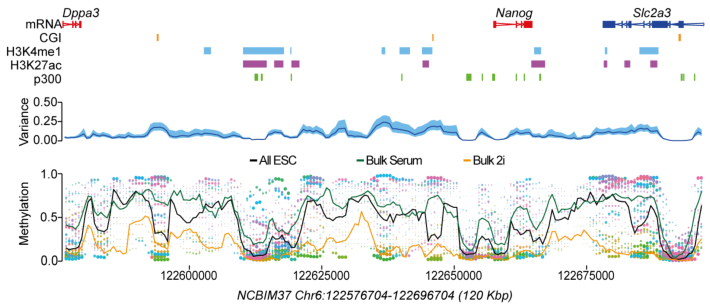
\includegraphics[width=1.0\textwidth]{zoom}
\caption[Estimated methylation rates for Nanog locus.]{Estimated DNA methylation rates using a sliding window in an example region containing the Nanog locus with some annotated features. Each single ESC is represented by a different color (bottom), and dot size is the inverse of estimation error. Mean methylation rate estimates across cells (black line, bottom) and cell-to-cell variance (blue line, middle; 95\% confidence interval in light blue) are shown. Methylation rates for `bulk serum' (green line) and `bulk 2i' (orange line) are superimposed (bottom).}
\label{fig:bs_zoom}
\end{figure}

We applied our method to estimate methylation rates in each ESC genome as well as the mean methylation rate and variance across all ESCs (\Cref{fig:bs_zoom}). By using our method for weighted clustering (\Cref{eq:bs_clust}), we identified two distinct clusters that represented the majority of 2i ESCs and serum ESCs (\Cref{fig:bs_clust}~(a)). Two outlier cells from the serum condition clustered with 2i ESCs, which implies that serum cultures contain `2i-like' ESCs and demonstrates the ability of scBS-seq to identify rare cell types in populations. To examine 5mC heterogeneity in ESCs in greater detail, we ranked sites by the estimated cell-to-cell variance (\Cref{eq:bs_var}) and repeated the cluster analysis for the 300 most variable sites (\Cref{fig:bs_top300}). The structure of the resulting clusters was broadly similar to what was observed based on genome-wide analysis, and all 300 variable sites followed the global trend of being more highly methylated in serum than 2i ESCs with high similarity between sites (\Cref{fig:bs_qc}~(b); \Cref{fig:bs_top300}). This observation is consistent with the genome-wide hypomethylation observed in ESCs grown in 2i medium~\citep{ficz_fgf_2013} and indicates that a major determinant of ESC heterogeneity is global methylation.

\begin{figure}[htbp!]
\centering
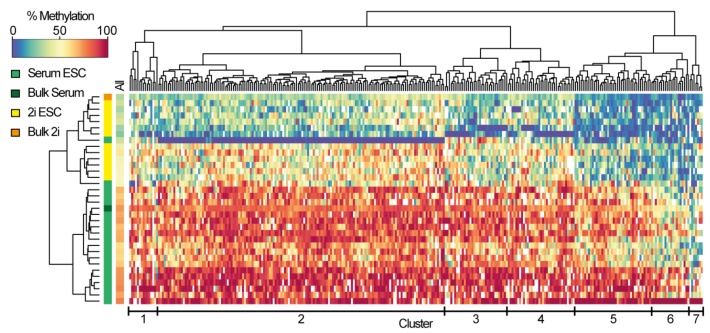
\includegraphics[width=1.0\textwidth]{top300}
\caption[Heatmap of 300 most variable sites.]{Heatmap for methylation rates of the 300 most variable sites among single-cell ESC samples. Cluster dendrograms for samples (left) and sites (top) are shown. The genome-wide average methylation rate is displayed in the left track (`all'). The main clusters of variable sites are indicated at the bottom.}
\label{fig:bs_top300}
\end{figure}

Our method also identified sites whose methylation varied more than the genome average, including sites with marked heterogeneity even among cells from the same growth condition (e.g. clusters 5 and 6 in serum ESCs; \Cref{fig:bs_top300}). Regions containing H3K4me1 and H3K27ac, marks associated with active enhancers, had the greatest variance in 5mC, whereas CGIs and intracisternal A-particle repeats had lower variance than the genome average (\Cref{fig:bs_clust}~(b)). These findings are consistent with observations that distal regulatory elements are differentially methylated between tissues and throughout development~\citep{stadler_dna-binding_2011,ziller_charting_2013,hon_epigenetic_2013}

\begin{figure}[htbp!]
\centering
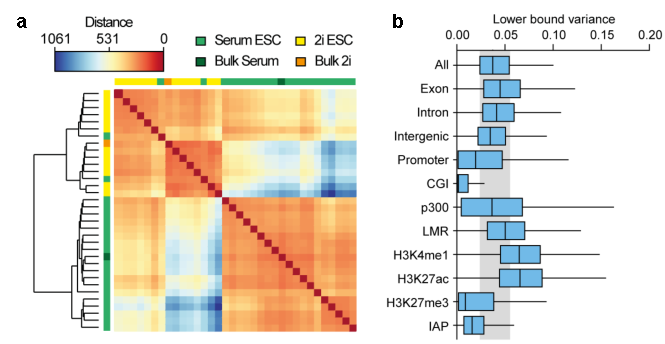
\includegraphics[width=1.0\textwidth]{clust}
\caption[Genome-wide clustering and estimated variance in genomic contexts.]{Genome-wide clustering and estimated variance in genomic contexts. (a) Genome-wide cluster dendrogram and distance matrix for all ESCs and bulk samples based on estimated methylation rates. Distance refers to the weighted Euclidean norm between estimated rates. (b) Variance of sites located in different genomic contexts. Boxes represent interquartile range with the median; whiskers correspond to 1.5 times the interquartile range. The shaded gray region indicates the interquartile range for all genome-wide sites.}
\label{fig:bs_clust}
\end{figure}

\section{Estimating associations between DNA methylation and gene expression} \label{sec:mt}

\ifpdf
    \graphicspath{{Chapter3/mt/Figs/Raster/}{Chapter3/mt/Figs/PDF/}{Chapter3/mt/Figs/}}
\else
    \graphicspath{{Chapter3/mt/Figs/Vector/}{Chapter3/mt/Figs/}}
\fi

We have shown that scBS-seq enables the exploration of intercellular heterogeneity in DNA methylation genome-wide. To further study the relationship between heterogeneity in DNA methylation and gene expression, we developed scM\&T-seq, a protocol for parallel profiling of DNA methylation and gene expression in single cells. In combination with scM\&T-seq, we developed methods for estimating associations between DNA methylation and gene expression in single cells, which will be described in the following.

\subsection{Parallel single-cell DNA methylation and gene expression profiling}

\citet{macaulay_g&t-seq:_2015} have recently developed G\&T-seq, a method for parallel genome and transcriptome sequencing within single cells. Importantly, G\&T-seq utilizes physical separation of RNA and DNA allowing bisulfite conversion of DNA without affecting the transcriptome. We now apply scBS-seq to genomic DNA purified according to the G\&T-seq protocol. Our scM\&T-seq protocol consists of isolating single cells, followed by physical separating DNA and RNA using the G\&T protocol (\Cref{fig:mt_proto}). DNA is bisfulfite treated and sequenced using scBS-seq to quantify DNA methylation of individual cells, and RNA is sequenced using scRNA-seq~\citep{jaitin_massively_2014} to quantify gene expression.

\begin{figure}[htbp!]
  \begin{minipage}[c]{0.65\textwidth}
    \centering
    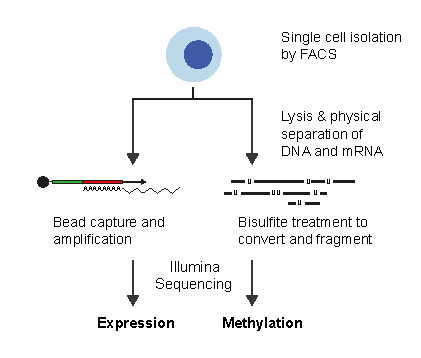
\includegraphics[width=1.0\textwidth]{proto}
  \end{minipage}
  \begin{minipage}[c]{0.32\textwidth}
    \caption[Schematic overview of the scM\&T-seq protocol.]{Schematic overview of the scM\&T-seq protocol. Single-cells are isolated by FACS sorting and extracted DNA separated from RNA using G\&T-seq. DNA is treated with bisulfite and sequenced using scBS-seq to quantify DNA methylation; RNA is amplified and sequences to quantify gene expression.}
    \label{fig:mt_proto}
  \end{minipage}
\end{figure}

We evaluated scM\&T-seq on mouse ESCs. In the presence of serum, these cells are characterized by high transcriptional and epigenetic heterogeneity. To investigate the link between epigenetic and transcriptional heterogeneity in ESCs, we performed scM\&T-seq on 76 individual serum ESCs and 16 ESCs grown in `2i' media, which induces genome-wide DNA hypomethylation.

To assess the quality of the scBS-seq data, we compared the resulting single-cell methylomes with the 20 serum and 12 2i ESCs that we profiled with stand-alone scBS-seq (\Cref{sec:bs_proto}). The genome-wide CpG coverage at matched sequencing depth was consistent across scM\&T-seq and scBS-seq (\Cref{fig:mt_qc}~(a)) and we found that scM\&T-seq covered a large proportion of sites in different genomic contexts with sufficient frequency to enable the analysis of epigenome heterogeneity across cells. As additional validation, we assessed the discrimination of serum and 2i ESCs by both stand-alone scBS-seq and scM\&T-seq, finding a similar degree of separation that was consistent with bulk datasets published previously~\citep{ficz_fgf_2013} (\Cref{fig:mt_qc}~(b)), with similar conclusions when using a joint hierarchical clustering across all cells (\Cref{fig:mt_clust}). Notably, the difference between protocols and biological batches had a substantially smaller effect (PC2, 3\% variance) than cell type differences (PC1, 48\% variance), and by combining data across cells, we found that both protocols yield genome-wide methylation profiles that accurately recapitulate bulk methylation profiles in the same cell type (\Cref{fig:mt_bulk}). Finally, we compared estimates of methylation heterogeneity in different genomic contexts, again finding good agreement between protocols (\Cref{fig:mt_var}). Taken together, these analyses provide confidence that the parallel scM\&T-seq method yields results that are in agreement with data from stand-alone scBS-seq.

\citet{macaulay_g&t-seq:_2015} has previously shown that the scRNA-seq data generated by the G\&T-seq method is of similar quality to that generated using the scRNA-seq protocol. We obtained an average of 2.7 million scRNA-seq reads per cell, and we excluded cells with fewer than 2 million mapped reads. In ESCs that met scRNA-seq quality-control criteria, we detected transcripts from between 4000 and 8000 genes exceeding one transcript per million, consistent with previous measurements made using the method (\Cref{fig:mt_qc_rna}).

\begin{figure}[htbp!]
\centering
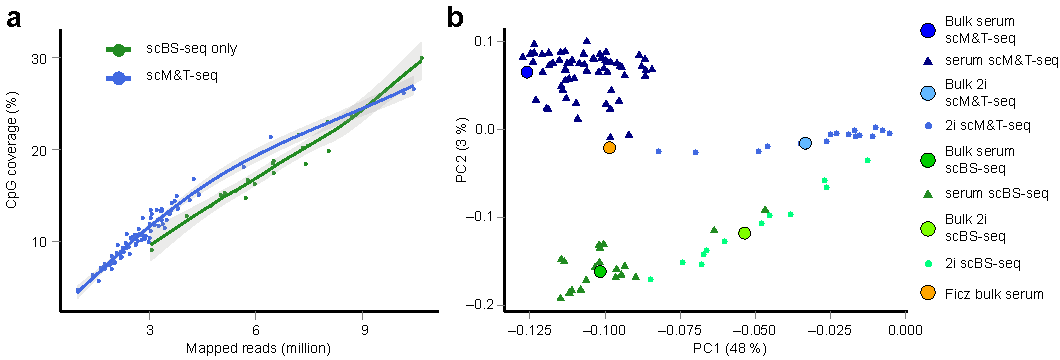
\includegraphics[width=1.0\textwidth]{qc}
\caption[Quality controls of scM\&T-seq protocol.]{Schematic overview of the scM\&T-seq protocol. (a) CpG coverage of single cells as a function of the number of mapped sequencing reads. Green: stand-alone scBS-seq, Blue: scM\&T-seq. (b) Joint principal component analysis of the methylomes (gene body methylation) of 61 serum ESCs (dark blue) and 16 2i ESCs (light blue) obtained using scM\&T-seq, as well as 20 serum ESCs (green) and 12 2i ESCs (yellow) sequenced using stand-alone scBS-seq. The solid circles correspond to synthetic bulk datasets form the same cells. For comparison, we also included a bulk serum ESC DNA methylation dataset~\citep{ficz_fgf_2013} (orange). Cell type explained a substantially larger proportion of variance (PC1, 48\%) than protocol (PC2, 3\%).}
\label{fig:mt_qc}
\end{figure}

For subsequent analyses, we focused on serum ESCs only since transcription and DNA methylation are uncoupled in 2i ESCs~\citep{ficz_fgf_2013,habibi_whole-genome_2013}. A comparison of the principal components derived from gene body methylation and gene expression revealed associations between some factors of variations of both data modalities (\Cref{fig:mt_cca}; \Cref{fig:mt_cca_cor}). However, a hierarchical clustering analysis of gene body methylation and gene expression for the 300 most variable genes revealed distinct clustering of cells when using either source of information (\Cref{fig:mt_heat}). This suggests that global methylome and transcriptome profiles yield complementary but distinct aspects of cell state. This is also consistent with previous observations that the transcriptome and methylome are partially uncoupled in serum ESCs~\citep{ficz_fgf_2013}.

\begin{figure}[htbp!]
\centering
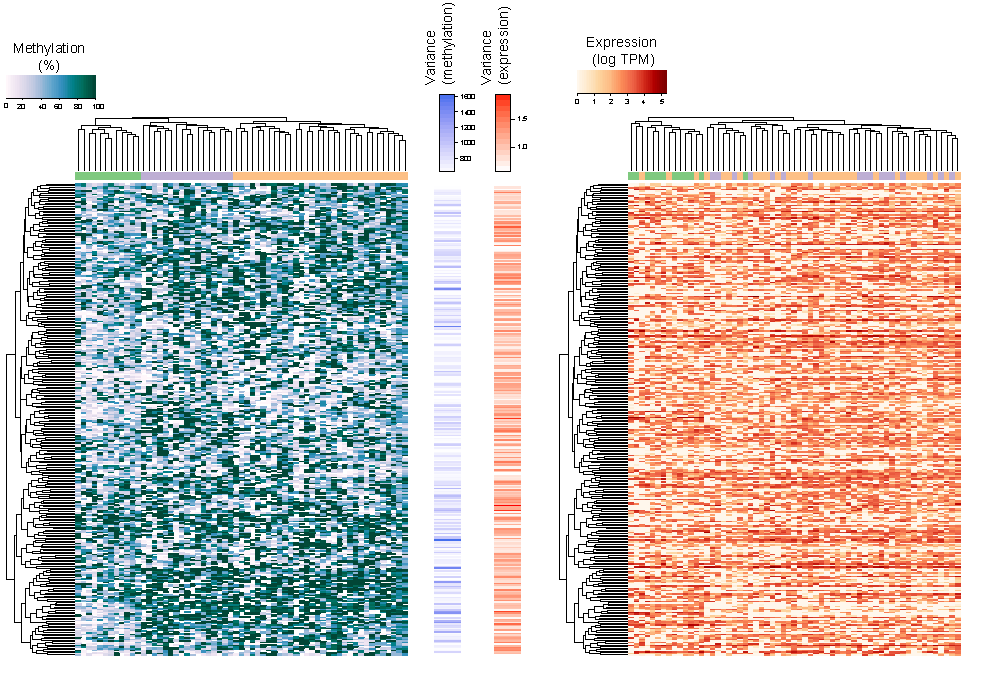
\includegraphics[width=1.0\textwidth]{heat}
\caption[Clustering analysis of transcriptome and methylome data.]{Clustering analysis of transcriptome and methylome data from 61 serum ESCs, considering gene body methylation (left) and gene expression (right) for the 300 most heterogeneous genes (based on gene body methylation). The order of genes was taken from an individual clustering analysis based on gene body methylation whereas cells were clustered separately either using DNA methylation or expression data, and coloured by methylation cluster. The bar plots in the center show the heterogeneity in DNA methylation (left) and gene expression (right).}
\label{fig:mt_heat}
\end{figure}


\subsection{Methods for estimating associations between DNA methylation and gene expression} \label{sec:mt_method}

\newcommand{\Xcov}{\operatorname{cov}}
\newcommand{\Xcor}{\operatorname{cor}}

\begin{figure}[htbp!]
\centering
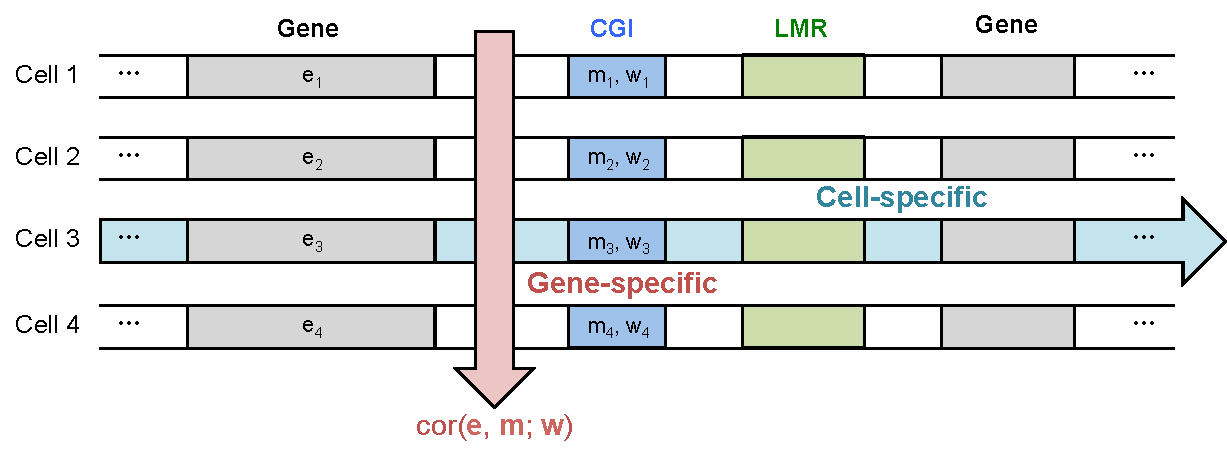
\includegraphics[width=1.0\textwidth]{method}
\caption[Schematic representation cell-specific and gene-specific correlation analysis between methylome and transcriptome.]{Schematic representation cell-specific and gene-specific correlation analysis between methylome and transcriptome. Cell-specific analysis is performed for a single cell or a bulk population of cells across multiple genes. Gene-specific analysis is performed for a single gene across multiple cells. The vector $e$ represents the expression rates of the considered gene for all cells, $m$ the mean methylation rates in the corresponding genomic context, and $w$ the number of covered CpG sites within that context. Associations were estimated by the weighted Pearson correlation $\Xcor(e, m; w)$ to account for differences in CpG coverage between cells.}
\label{fig:mt_method}
\end{figure}

Previous studies on data from bulk sequencing protocols estimated correlations between methylome and transcriptome in a bulk population of cells across multiple genes (\Cref{fig:mt_method}). In contrast, scM\&T-seq separates individual cells and hence enables estimating associations for a particular gene across multiple cells. Let $e$ be a vector with expression rates of cells for a particular gene, $m$ be methylation rates of the associated region, and $w$ be weights corresponding to the number of covered CpGs sites within the region. Then we estimated associations using weighted Pearson correlation $\operatorname{cor}(e,m;w)$ between gene-expression $e$ and methylation $m$:
\begin{align} \label{eq:mt_wcor}
  \Xcor(e,m;w)=\frac{\Xcov(e,m;w)}{\sqrt{\Xcov(e,e;w)\Xcov(m,m;w)}}
\end{align}
Here, $\Xcov(x,y;w)$ is the weighted covariance
\begin{align}
  \Xcov(x,y;w)=\sum_i \frac{w_i (x_i-m(x;w))(y_i-m(y;w))}{\sum_i w_i },
\end{align}
and $m(x;w)$ the weighted arithmetic mean:
\begin{align}
  m(x;w)=\frac{\sum_i x_i w_i}{\sum_i w_i}
\end{align}
By computing weighted correlations, we accounted for differences in CpG coverage between cells. We considered all possible relationships between genes and methylated regions within 10~kbp of the gene (upstream and downstream of gene start or stop). We performed two-sided Student's t-tests to test for non-zero correlations, and adjusted p-values for multiple testing for each context using the Benjamini-Hochberg procedure.

We considered gene expression levels on a logarithmic scale using log10 normalized TPM counts. We estimated binary single-base pair CpG methylation states by the ratio of methylated read counts to total read counts. We further estimated the methylation rate in different genomic contexts, such as gene body, promoter, or enhancer annotations, as the mean CpG methylation rate within the region defined by the context.

We discarded genes with low expression levels or low expression and methylation variability between cells, following the rational of independent filtering~\citep{bourgon_independent_2010}. First, a minimum expression level (at least 10 TPM counts) in at least 10\% of all cells was required. From these, the 7500 most variable genes were considered for analysis. Second, methylated regions were required to be covered by at least one read in at least 50\% of all cells.


\subsection{Associations between DNA methylation and gene expression in different genomic contexts} \label{sec:mt_results}

Using weighted Pearson correlation (\Cref{eq:mt_wcor}), we tested for associations between expression of individual genes and DNA methylation variation at several genomic contexts. We identified a total of 1493 associations ($\FDR<0.1$; \Cref{fig:mt_gene_volcano}), which were robust when using a bootstrapping approach to subsample the set of cells. We found both positive and negative associations, highlighting the complexity of interactions between the methylome and transcriptome~\citep{dey_integrated_2015}. While methylation of non-CGI promoters is known to be associated with transcriptional repression, the role of enhancer methylation is less clear. Accordingly, negative correlations between DNA methylation and gene expression were predominant for non-CGI promoters, whereas positive and negative associations were more balanced in distal regulatory elements including LMRs (\Cref{fig:mt_gene_volcano}; \Cref{fig:mt_gene_r}; \Cref{fig:mt_gene_volcano_all}). Interestingly, associated genes were enriched for known pluripotency and differentiation genes~\citep{kolodziejczyk_single_2015} ($\FDR<0.01$, Fisher's exact test). Our results provide the first evidence that heterogeneous methylation of distal regulatory elements, e.g. LMRs, accompanies heterogeneous expression of key pluripotency factors in stem cell populations~\citep{lee_reprogramming_2014}.

\begin{figure}[htbp!]
\centering
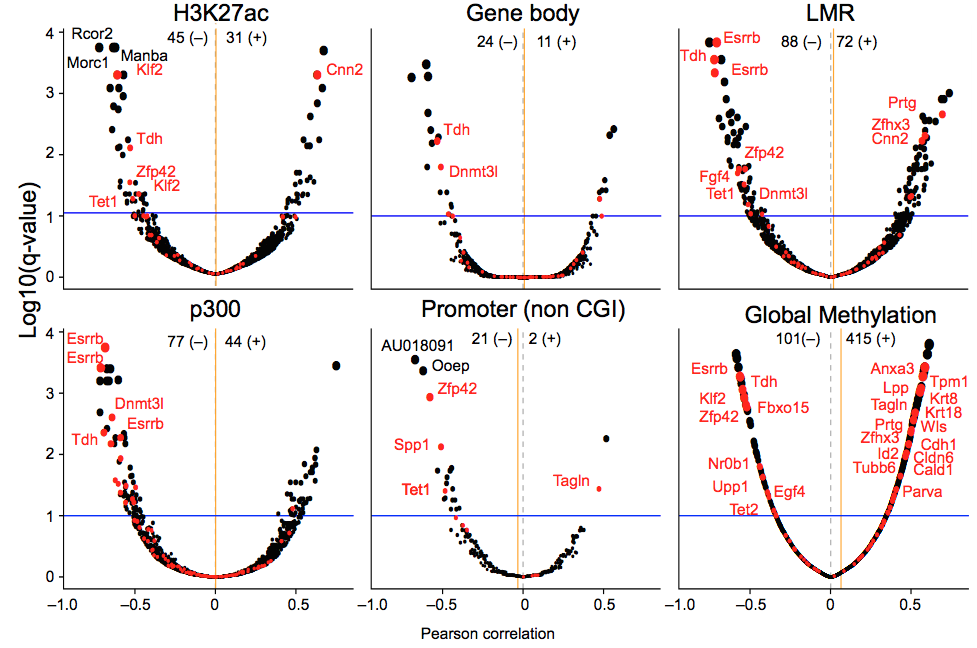
\includegraphics[width=0.8\textwidth]{gene_volcano}
\caption[Volcano plots of correlation coefficients.]{Volcano plots of correlation coefficients (Pearson's $r^2$) from association tests between gene expression heterogeneity of individual genes and DNA methylation heterogeneity in alternative genomic contexts. Shown is the correlation coefficient for every gene (x-axis) versus the adjusted p-value (using Benjamini-Hochberg correction; y-axis). The size of dots corresponds to the adjusted p-value. A set of 86 known pluripotency and differentiation genes are highlighted in red. The blue horizontal line corresponds to the $\FDR=0.1$ significance threshold. The total number of significant positive (+) and negative (–) correlations ($\FDR<0.1$) for each annotation is shown in the header of each panel. The orange vertical bar corresponds to the average correlation coefficient across all genes for a given context.}
\label{fig:mt_gene_volcano}
\end{figure}

As an example, \cref{fig:mt_zoom} shows the association map of Esrrb--a known key regulator gene in pluripotency networks~\citep{papp_pluripotency_2012}. Expression of Esrrb negatively correlated with the methylation of several LMR and p300 sites overlapping `super enhancers' in the genomic neighbourhood~\citep{whyte_master_2013}, providing evidence for the regulatory importance of Esrrb. We also found 516 genes whose expression correlated with the overall methylation level ($\FDR<0.1$), indicating substantial links between transcriptional heterogeneity and global methylation levels (\Cref{fig:mt_gene_volcano}).

\begin{figure}[htbp!]
\centering
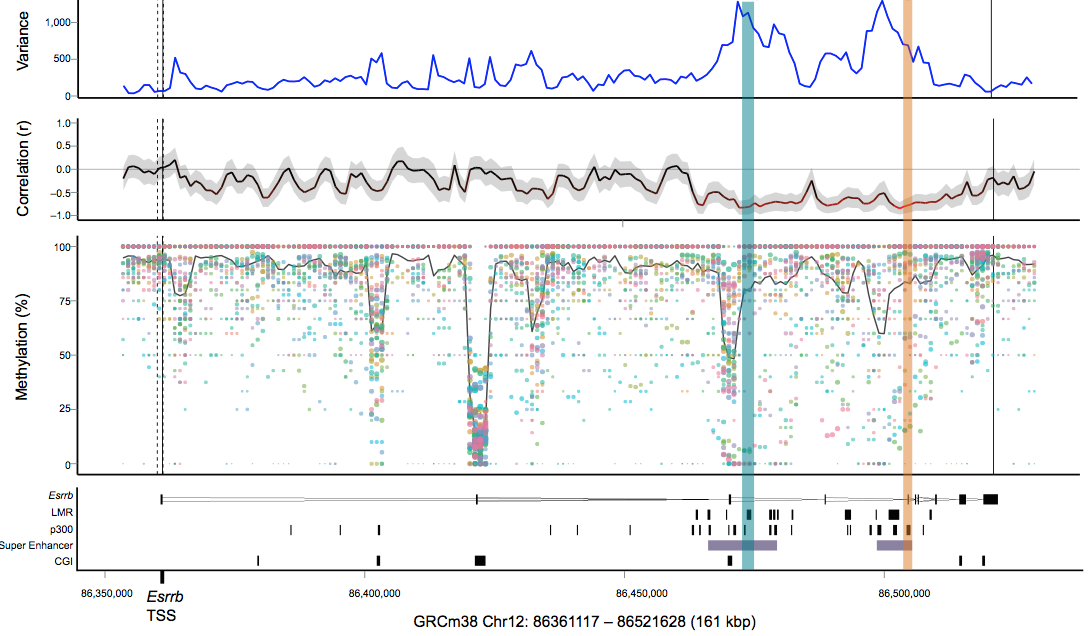
\includegraphics[width=1.0\textwidth]{zoom}
\caption[Representative zoom-in view for the gene Esrrb.]{Representative zoom-in view for the gene Esrrb. From bottom to top, shown is: the annotation of the Esrrb locus with LMR, p300, super enhancer and CGI sites indicated; the estimated methylation rate of $3~kbp$ windows for each cell with the size of dots representing the CpG coverage and the solid line indicating the weighted mean methylation rate across all cells; the correlation between the methylation rate and Esrrb expression for each region coloured by the strength of the correlation and with the shaded area corresponding to the 95\% confidence interval of the correlation coefficient; and the estimated weighted DNA methylation variance between cells. The vertical bars denote the location of a p300 (yellow) and LMR (blue) region, in which DNA methylation is significantly associated with gene expression.}
\label{fig:mt_zoom}
\end{figure}

In addition to between-cell analyses, scM\&T-seq can be used to correlate the methylome and transcriptome between genes in individual cells (\Cref{fig:mt_method}; \Cref{fig:mt_cell}), analogously to studies in cell populations. We found that correlation between methylation and gene expression varied substantially between cells but was consistent in direction with matched RNA-seq and BS-seq data from a population of cells~\citep{ficz_fgf_2013}. Again, this attests to scM\&T-seq being sufficiently accurate to reliably study epigenome-transcriptome linkages. Our results also point to the possibility of heterogeneity between cells in the degree of coupling between the methylome and the transcriptome. Although we have ruled out obvious confounding factors, such as average methylation rate and sequence coverage (\Cref{fig:mt_cell_r_mean}; \Cref{fig:mt_cell_r_cov}), more data will be required to understand possible technical components in these linkages.

\begin{figure}[htbp!]
\centering
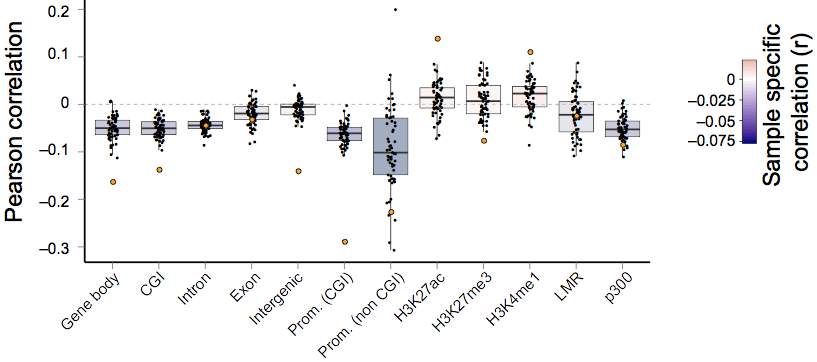
\includegraphics[width=1.0\textwidth]{cell}
\caption[Cell-specific correlation analysis]{Cell-specific association analysis, estimating correlations between DNA methylation in different genomic contexts and gene expression in individual cells. For each annotation, shown are box plots of methylation-expression correlations for all variable genes in single cells, with the correlation obtained from matched RNA-seq and BS-seq of a bulk cell population superimposed (orange circles).}
\label{fig:mt_cell}
\end{figure}



\section{Discussion}

We have first presented scBS-seq for profiling DNA methylation in single cells and a statistical model for quantifying methylation heterogeneity in cell populations at a genome-wide scale. We demonstrated that our approach detects rare cell types in populations and identifies genomic regions with high methylation heterogeneity that are functionally important during cell differentiation.

We further extended our protocol for parallel profiling of the methylome and transcriptome from the same single cell, allowing the relationship between DNA methylation and expression to be explored. We confirmed a negative association between non-CGI promoter methylation and transcription in single cells and identified both positive and negative associations at distal regulatory regions. We found the expression levels of many pluripotency factors, e.g. Esrrb, to be negatively associated with DNA methylation. Furthermore, we demonstrated that the strength of the connection between methylome and transcriptome can vary from cell to cell.

We used principal component analysis to investigate the factors of variations of DNA methylation and gene expression. To better understand the relation between these factors and to distinguish between factors that drive variations either in DNA methylation or gene expression, future studies may consider advanced statistical methods such as canonical correlation analysis or collective matrix factorization.

In our study, we only considered correlations between genes and genomic regions with a maximum genomic distance of 10~kbp. An important area of future research is to investigate trans-associations between DNA methylation and gene expression. For this, chromatin contact information from Hi-C experiments can be considered to identify distal genomic regions that are in close spatial proximity with a certain gene.

We estimated mean methylation rates in genomic context by averaging and used weighted Pearson correlation to account for incomplete CpG coverage. More sophisticated methods to estimate the mean methylation rate in genomic context from low-coverage data may reveal stronger associations between DNA methylation and gene expression. These include methods for imputing CpG methylation in single cells, which will be discussed in the following chapter.
